\documentclass[a4paper,11pt]{article}
\usepackage{graphicx}
\usepackage[T1]{fontenc} % codifica dei font in uscita
\usepackage[utf8]{inputenc} % lettere accentate da tastiera
\usepackage[italian]{babel} % lingua principale del documento
\usepackage{latexsym}
\usepackage{url}
\usepackage [a4paper, top=2.5cm, bottom=2.5cm, left=1.5cm, right=1.5cm, bindingoffset=8mm] {geometry}

% inizio documento

\begin{document}

\begin{center}
\textsc{\Huge Esperienza I}\\[0.5cm]
\large
\title{ESPERIENZA 3}

%\emph{\large\textbf{Autori}}\\ \\ 
Michele \textsc{Pedrotti}
Luigi \textsc{Bassini}
Nicola \textsc{Trevisson}
Giacomo \textsc{Alberini}\\
\today
\end{center}

\section{Introduzione}
Scopo dell'esperienza è quello di misurare l'andamento della pressione durante la fase di svuotamento di un volume di aria, utilizzando diverse pompe e confrontando i risultati. Successivamente si è cercato di misurare alcune caratteristiche di gas noti e ignoti applicando la legge di stato dei gas ideali. 
\section{Confronto pompe a vuoto}

Inizialmente il gruppo si è preoccupato di misurare il volume del contenitore usato nell'esperienza. Per stimare questa grandezza la bottiglia è stata riempita di acqua e quindi è stato misurato il valore del volume in litri con un cilindro graduato. Il valore ottenuto è il seguente:
$$2.775  ~l\pm 0.009 ~l$$
Il passo successivo consisteva nel creare il vuoto nella camera utilizzando due tipi di pompe: una manuale e l'altra meccanica. \\
Per la prima i risultati sono stati riassunti in un grafico che mostra l'andamento della pressione (misurata con un manometro differenziale al mercurio) al variare del numero di pompaggi manuali effettuati. Con la seconda si è preferito invece sostiuire al numero di pompaggi il tempo misurato in secondi avvalendosi di un cronometro. Sono stati dunque prodotti i due seguenti grafici.
\\

\begin{figure}[htbp]
\centering
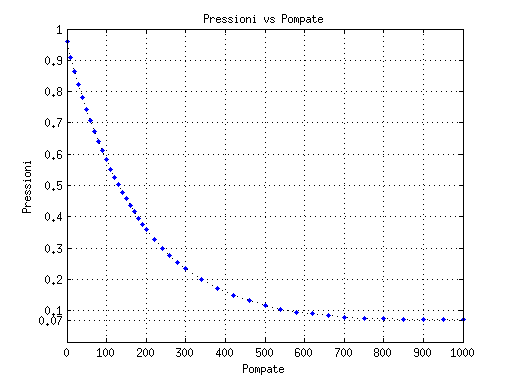
\includegraphics[width=15cm]{prexpomp.png}
\end{figure}


\begin{figure}[htbp]
\centering
\includegraphics[width=15cm]{grafico_Pt.png}
\end{figure}


NOTA : Per la loro ridotta dimensione le barre di errore non risultano visibili all'interno della risoluzione del grafico. Si può anche notare un leggero flesso all'interno del secondo grafico legato alla repentina varizione di pressione che ha procurato un'oscillazione della colonnina di mercurio.\\


Come si può notare, entrambi i grafici mostrano un'andamento esponenziale che tende a un valore particolare di pressione, caratteristico dello strumento utilizzato. \\
Il valore limite delle due pompe, apprezzabile anche dai grafici, vale 7000 Pa $\pm 300$ Pa per la pompa manuale, e 1300 Pa $\pm 300$ Pa per la pompa meccanica.\\
Si nota anche che la pompa meccanica (azionata da un motore elettrico) raggiunge un valore di pressione finale minore rispetto a quella manuale.
L'andamento, in entrambi i grafici, sembra essere del tipo: $P=P\ped{0}+ae^{bx}$, dove P è la pressione, $P\ped{0}$ la pressione limite valutata sperimentalmente, a e b i parametri della curva (è da notare che il parametro b dovrà evidentemente avere un valore negativo), e x una variabile indicante il numero di pompate nel primo caso e il tempo nel secondo.

I risultati dei due fit sono sintetizzati nella seguente tabella.\\
\begin{center}
\begin{tabular}{|c|c|c|c|}
\hline $Tipo$ $di$ $pompa$ & $Pressione$ $limite$ & $a[Pa]$ $\pm$ $\delta a$ & $b$ $\pm$ $\delta b$ \\ 
\hline Pompa Manuale & 7000 $Pa \pm 300 Pa$ & 0.89$\pm 0.04$  &-0.0056 $\pm0.0003$  \\ 
\hline Pompa Meccanica & 1300$Pa \pm 300Pa$ & 0.84$\pm$0.04 & -0.152$\pm$0.007 \\ 
\hline 
\end{tabular} 
\end{center}
NOTA: Per quanto riguarda l'unità di misura sul parametro b, esse sono diverse nei due casi. Per la pompa meccanica $[b]=[s^{-1}]$ mentre per la pompa manuale b è un numero adimensionale.

\subsection{Calcolo della densità dell'aria}
Per definizione, la densità è rappresentata dal rapporto tra massa e volume. Avendo già calcolato precedentemente il volume della bottiglia in cui è contenuto il gas, abbiamo proceduto valutando la massa del gas. Questo valore si può ottenere per differenza tra il peso della bottiglia vuota (1564.8g $\pm 0.05$g), e il peso della bottiglia in cui è presente gas d'aria alla pressione di 3 Atm (1574.4g $\pm 0.05$g).\newpage
 Il valore ottenuto è: 9.6g $\pm 0.05$ g.
Ne segue che la densità dell'aria a $3 ~atm$ è  $d= m/V= 3.46 kg/m^3 \pm 0.02kg/m^3$  

\section{Calcolo del peso molare di alcuni gas}
Successivamente si sono calcolati i valori di massa molare di alcuni gas, utilzzando la legge di stato dei gas perfetti.
Dopo aver calcolato la massa della bottiglia in cui era stato fatto il vuoto utilizzando la pompa meccanica, per differenza sono state calcolate le masse dei diversi gas.
Conoscendo la massa del gas, per conoscere la massa molare dobbiamo conoscerne il numero di moli contenute nel volume della battiglia. Utilizzando la relazione $PV=nRT$ , otteniamo $n=PV/RT$, dove P è la pressione all'interno della bottiglia misurata attraverso il manometro differenziale e con valore 299000 Pa $\pm500$ Pa, V il volume della bottiglia, R la costante universale dei gas e T la temperatura ambientale al momento dell'esperimento).E' da notare che, poichè il manometro utilizzato per misurare la pressione all'interno della bottiglia è un manometro di tipo differenziale, è stato necessario misurare la pressione atmosferica al momento dell'esperimento. Questo valore, rimasto costante durante il pomeriggio, era di 97300 Pa $\pm70$ Pa, ed è stato misurato attraverso un manometro a tubi di vetro. Successivamente, dalla relazione M$\ped{mol}$=$m/n$ otteniamo quindi la massa molare del gas. I risultati ottenuti sono quindi stati riportati nella seguente tabella: 
\hspace{-140pt}

\begin{center}
\begin{tabular}{|c|c|c|c|c|}
\hline \rule[-2ex]{0pt}{5.5ex} $Gas$ & $Massa [g]$ & $Temperatura [^\circ{C}]$ & $Massa Molare [g/mol]$ & $M. Mol. Tabulato [g/mol]$ \\ 
\hline \rule[-2ex]{0pt}{5.5ex} Elio & $1.3 \pm 0.05$ & $22.7 \pm 0.1$ & $3.9 \pm 0.2$ & 4.002 \\ 
\hline \rule[-2ex]{0pt}{5.5ex} Azoto & $9.2 \pm 0.05$ & $22.4 \pm 0.1$ & $27.9 \pm 0.5$ & 28.034 \\ 
\hline \rule[-2ex]{0pt}{5.5ex} Ignoto & $13.1 \pm 0.05$ & $22.3 \pm 0.1$ & $39.7 \pm 0.7$ & ? \\ 
\hline \rule[-2ex]{0pt}{5.5ex} CO\ped2 & $15.2 \pm 0.05$ & $22.5 \pm 0.1$ & $46.1 \pm 0.8$ & 44.010 \\ 
\hline 
\end{tabular}
\end{center}
\vspace{40pt}

NOTA: nella tabella non sono stati inseriti i volumi, la pressione e il numero di moli perche a valori costanti.\\

Notiamo che, per l'Elio e l'Azoto i valori calcolati sono compatibili con i valori presenti sulla Tavola periodica degli Elementi. \\
Per quanto riguarda il terzo gas, partendo dal presupposto che esso sia effettivamente un \emph{singolo} gas e non un miscuglio di diversi elementi, considerando le condizioni ambientali in cui si è effettuato l'esperimento, l'unico elemento combatibile con i dati tabulati è il gas nobile Argon ($39.94g/mol$). \\ Con i dati in nostro possesso, comunque, non è possibile risalire con certezza al reale contenuto della bottiglia. 
\\
\\
Infine si è notato che il valore di massa molare del biossido di carbonio da noi trovato era \emph{incompatibile} rispetto al valore noto. \\
Evidentemente non è possibile utilizzare la legge di stato dei gas perfetti per approssimare il comportamento di tale gas. Questo perchè la molecola di biossido di carbonio non gode di quelle proprietà fisiche (struttura puntiforme, basse interazioni intramolecolari, densità uniforme, ecc) che permettono di utilizzare tale relazione per stimarne il comportamento.
\end{document}